\section{Results}

This section examines necessary steps to apply the showcases stated in \autoref{sec:showcases-1} with \linkerd{}, how the results look like and some pitfalls we have overcome.

Since functionality and APIs vary in time, the following table shows the versions of technologies we use:
\begin{table}[h]
\centering	
\begin{tabular}{c|c}
	Technology & Version \\\hline
	\textsc{Docker} & 20.10.3\\\hline
	\textsc{Minikube} & 1.17.1\\\hline
	\kubernetes & 1.20.2\\\hline
	\linkerd & 2.9.3 \\
\end{tabular}
\vspace{0.25mm}
%\caption{Comparison between Isto and \textsc{Linkerd}}
\label{tab:versions}
\end{table}

Services are built into \textsc{Docker}-images.
To use only one machine for development we used \textsc{Minikube}.
Within this \kubernetes{} and \linkerd{} run.

\subsection{Showcases Implementation}
With the exception of "Acess Policies" we implemented and controlled with \linkerd{} the challenges stated in \autoref{sec:showcases-1}.

\subsubsection{Encryption}
From the second that a service is injected by \linkerd{} and applied to the cluster, all communication to that service is automatically encrypted.
This holds not only for our self-implemented communication but also for metrics- and tap-services.
Since the communication is proxied by \linkerd{} it activates certificate distribution and encryption out-of-box.

If you don't want to use this feature, you can disable by overwriting the \linkerd{} configuration.
The following command will generate an updated YAML-configuration you can apply in \kubernetes{}.
\begin{lstlisting}
linkerd upgrade \
  --disable-identity \
  --disable-tap
\end{lstlisting}
Note: Once this configuration is applied, there will be no encryption neither in communication between services nor in tap- and metrics-services.

\subsubsection{Canary Deployment}
\label{sec:canary-result}
In first place we have to deploy a new version of the \textsc{name-service} next to the existing one.
The deployment is done the same way but with a different name (\lstinline|nameapi-v2|).
New Version of \textsc{name-service} is similar to the old one but returns a different string (forename \textit{and} surname) while API stays the same.
There are no changes in \textsc{hello-world-service} necessary.

Until now the new version is not used.
We have to define a traffic split showed in \autoref{lst:traffic-split}.

\begin{lstlisting}[caption={YAML configuration of 90/10 traffic split. 90\% of requests are routed to \lstinline|nameapi| and 10\% to \lstinline|nameapi-v2|.}, label={lst:traffic-split}]
apiVersion: split.smi-spec.io/v1alpha1
kind: TrafficSplit
metadata:
	name: nameapi-split
spec:
	service: nameapi
	backends:
	- service: nameapi
		weight: 90
	- service: nameapi-v2
		weight: 10
\end{lstlisting}

In the \lstinline|spec|-section we define two backends for the service \lstinline|nameapi|.
The argument \lstinline|weight| defines a split ratio.
90\% of traffic should be routed to the existing service with the name \lstinline|nameapi|, 10\% to the new one \lstinline|nameapi-v2|.

Right after applying this configuration, \linkerd{} dashboard shows a new section for traffic splits.
In \autoref{fig:results-traffic-split-weights} \linkerd{} visualizes the routed requests.
We can see the defined weights and the current requests per second (RPS), that are split according.

\begin{figure}
	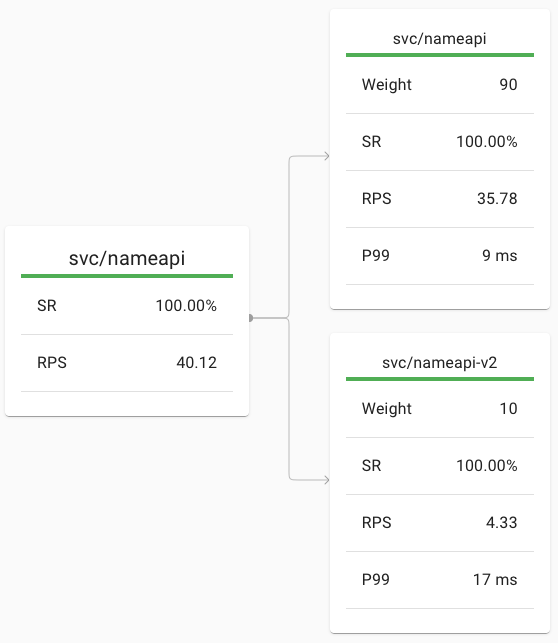
\includegraphics[width=\columnwidth]{img/results-traffic-split-weights}
	\caption{\linkerd{} dashboard displays the weights of the 90/10 traffic split.}
	\label{fig:results-traffic-split-weights}
\end{figure}

The \textsc{hello-world-service} stays unchanged, but requests the new version of \textsc{name-service} every tenth request without knowing.
The deployment section of \textsc{hello-world-service} in \linkerd{} dashboard now renders a delegation tree pictured in \autoref{fig:results-traffic-split-tree} showing that \textsc{hello-world-service} requests both versions of \textsc{name-service}.

\begin{figure}
	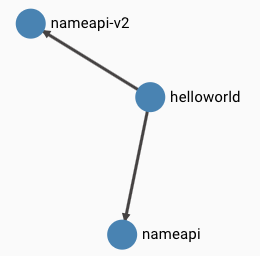
\includegraphics[width=.4\columnwidth]{img/results-traffic-split-tree}
	\centering
	\caption{Delegation tree of \textsc{hello-world-service} after traffic split.}
	\label{fig:results-traffic-split-tree}
\end{figure}




\subsubsection{Access Policies}
TBD

\subsubsection{Load Balancing}
\label{sec:load-result}
To show the integrated load balancing of \linkerd{} we defined three replicas of the \textsc{goodbye-world-service}.
Therefore we set In the deployment configuration at the \lstinline|spec|-section the count of replicas up to three	 (\lstinline|replicas: 3|).
Now \kubernetes{} will provide three pods running the \textsc{goodbye-world-service}.
Since we injected the configuration file by \linkerd{} all replicas are within the service mesh and load balancing takes place out-of-box.

\autoref{fig:results-load-balance} shows the pods list of \linkerd{} dashboard in the deployment view of \textsc{goodbye-world-service}.
We can see that requests are balanced equally to each replica.

\begin{figure}
	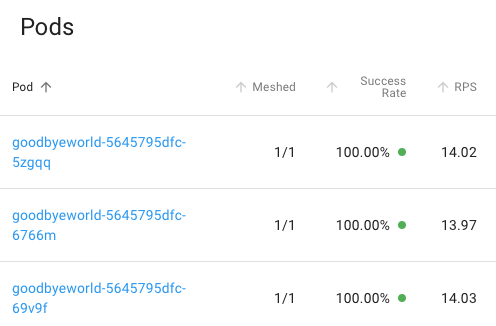
\includegraphics[width=\columnwidth]{img/results-load-balance}
	\caption{The \textsc{goodbye-world-service} deployment shows all three replicas balancing the request-load.}
	\label{fig:results-load-balance}
\end{figure}

\subsubsection{Central Monitoring and Logging}
As we can see \linkerd{} comes with a dashboard showing the current state of the service mesh.

\begin{itemize}
	\item Monitoring comes "out-of-box"
	\item as it was shown in images in \autoref{sec:canary-result} and \autoref{sec:load-result}
	\begin{itemize}
		\item \linkerd{} brings \textsc{Prometheus} and \textsc{Grafana}
		\item  Now we can see \textbf{who} is talking \textbf{how much} to \textbf{whom}
		\item Maybe show a call-tree from linkerd-dashboard?
	\end{itemize}

	\item There was an own log-command by \linkerd{} (\lstinline|linkerd logs|)
	\item Logging (\lstinline|linkerd logs|) by linkerd was removed, since it was the same as logs from \lstinline|kubectl|\\
	(\url{https://github.com/linkerd/linkerd2/discussions/5790})
	\item How to use \lstinline|kubectl|?\\
		\lstinline|kubectl logs <pod> <service>|
	\item here the \lstinline|bash-completion| is very useful (see appendix)
	\item often read: \textsc{Loki} as logging solution...?
	\begin{itemize}
		\item easy to embed into  Grafana
	\end{itemize}
\end{itemize}


\subsection{Pitfalls}
...and lessons learned?

\begin{itemize}
	\item it's abit more than \linkerd{}.
	\item We will need to know about \lstinline|kubectl|.
	\item we weren't able to apply access policies
\end{itemize}
\begin{itemize}
	\item \linkerd{} says, it'll need only 2GB of RAM 
	\begin{itemize}
		\item that was not enough. K8s was crashing
		\item With 4 GB it works
	\end{itemize}

	\item Minikube
	\begin{itemize}
		\item use command to build docker images into minikube-environment to be available in K8s.
	\end{itemize}

	\item Bring some time...
	\item There os no way to use \linkerd{} without \kubernetes{}. You'll have to learn some \kubernetes{} as well ;)
	\item use bash-completion
	\item Use ssh-port-forwarding to communicate with dashboard on VPS	
\end{itemize}

For further details on the setup, configuration and usage, see the appendix.